\newpage

\section{Durchführung}
\label{sec:Durchführung}

\begin{figure}
  \centering
  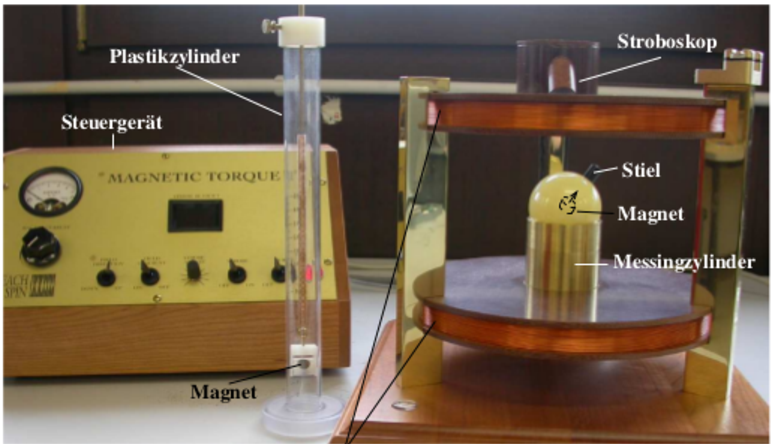
\includegraphics[width=0.8\textwidth]{content/images/bild1.pdf}
  \caption{Versuchsanordnung.}
  \label{fig:1}
\end{figure}

In eine Billardkugel ist mittig ein kleiner Stabmagnet mit
dem zu bestimmenden $\mu_{Dipol}$,welches entlang
des auf (Abb.\ref{fig:1}) zu erkennenden Stiels
gerichtet ist, eingelassen. Im Zentrum der Helmholtzspule
ist eine Vorrichtung, welche der Billardkugel erlaubt nahezu
reibungsfrei auf einem Luftkissen zu gleiten.
Die Ausmaße der verwendeten Helmholtzspule sind N = 195 Windungen mit
einem Abstand von $d = 0.138m$ und einem Spulenradius von $R = 0.109m$.
Das in (Abb.\ref{fig:1}) zu sehende Steuergerät steuert das Stroboskop, den Spulenstrom,
 Feldrichtung und -gradient.


 \subsection{Durchführung der Messung per Gravitation}
 \label{ssec:DurchGrav}

 \begin{figure}
   \centering
   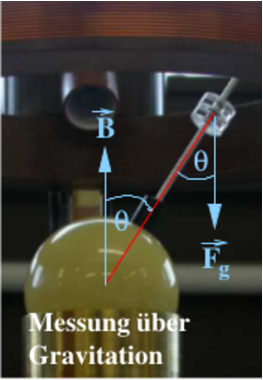
\includegraphics[width=0.3\textwidth]{content/images/bild3.pdf}
   \caption{Messung per Gravitation.}
   \label{fig:2}
 \end{figure}

In den Stiel wird eine dünne Aluminiumstange
gesteckt, an welche ein kleines Gewicht der Masse $m$ angebracht wird.
Der Abstand $r$ des Gewichtes zum Schwerpunkt der Kugel ist variabel.
Das Drehmoment der Gravitationskraft und des Magnetfeldes sind entgegengesetzt.
Zur Messung wird das Luftkissen aktiviert, sodass die Kugel möglichst
reibungsfrei gelagert ist und die Aluminiumstange samt Masse an der Kugel angebracht.
Dann wird der Spulenstrom $I_{\text{Spule}}$ solange erhöht bis sich ein Gleichgewicht einstellt und
$r$ und $I_{\text{Spule}}$ notiert. Es werden 10 Messungen mit 10 verschiedenen $r$ vorgenommen.

\subsection{Durchführung der Messung per Schwingungsdauer}
\label{ssec:DurchSchw}

Bei dieser Messmethode wird die Billardkugel in der homogenenen magnetischen Flussdichte $\vec{B}$ durch
Auslenkung in Schwingung versetzt und oszilliert harmonisch. Zur Messung wird das Magnetfeld und das Luftkissen aktiviert.
Daraufhin wird der Stiel ausgelenkt und die Dauer von 10 Perioden $T_{10}$ und der Spulenstrom $I_{\text{Spule}}$ notiert.
Dies wird für 10 verschiedene $I_{\text{Spule}}$ durchgeführt.

\subsection{Durchführung der Messung über Präzessionsdauer}
\label{ssec:DurchPraez}

\begin{figure}
  \centering
  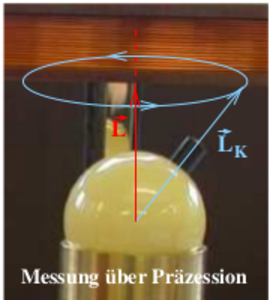
\includegraphics[width=0.3\textwidth]{content/images/bild4.pdf}
  \caption{Messung per Präzessionsdauer.}
  \label{fig:3}
\end{figure}
Diese Messmethode funktioniert durch das Einwirken einer
äußeren Kraft auf die Drehachse der rotierenden Billardkugel.
Die äußere Kraft ist in diesem Fall durch das
einwirkende Magnetfeld gegeben.
Die Kugel wird mit dem Stiel als Drehachse zum rotieren
gebracht und dann ausgelenkt, hierbei sollte
die Rotation stabil bleiben, da sonst Nutation beim einschalten
des Magnetfeldes entsteht. Das Stroboskop wird auf eine
Frequenz zwischen 4Hz und 6Hz eingestellt.
Das Magnetfeld wird eingeschaltet sobald die Markierung auf dem
Stiel unter dem Licht des Stroboskops statisch erscheint. Damit beginnt
die Präzessionsbewegung und die Umlaufszeit $T$ der Präzession wird gemessen.
Der Spulenstrom $I_{\text{Spule}}$ und die Umlaufzeit werden notiert. Pro
$I_{\text{Spule}}$ wird die Umlaufzeit drei mal gemessen und dies für
10 verschiedene $I_{\text{Spule}}$ wiederholt.





\newpage
